%!TEX program = xelatex

\documentclass[UTF8]{ctexart}
\usepackage{ctex}

\CTEXsetup[format={\Large\bfseries}]{section}

\usepackage[version=3]{mhchem} % Package for chemical equation typesetting
\usepackage{siunitx} % Provides the \SI{}{} and \si{} command for typesetting SI units
\usepackage{graphicx} % Required for the inclusion of images
\graphicspath{{assets/}}
\usepackage{natbib} % Required to change bibliography style to APA
\usepackage{amsmath} % Required for some math elements 
\usepackage[hidelinks]{hyperref}
\usepackage{makecell} % 3 Packages for flexible tabular
\usepackage{multirow}
\usepackage{multicol}

\usepackage{geometry}% 版面大小
\geometry{a4paper,scale=0.7}

\usepackage{fontspec}

\setCJKfamilyfont{hwxk}{STXingkai}% 字体
\newcommand{\hwxk}{\CJKfamily{hwxk}}

\usepackage{fancyhdr}% 页眉页脚
\fancypagestyle{EE_AnalogExp_template}{
    \fancyhead[L]{\Large {\hwxk 南京大学电子科学与工程学院}}
    \fancyhead[R]{模拟电路实验报告}
    \fancyfoot[c]{- \thepage \ -}
    \renewcommand\footrulewidth{0pt}
}

% 4级目录
\setcounter{secnumdepth}{4}
\setcounter{tocdepth}{4}

\usepackage{graphicx} % Packages for figures
\usepackage{caption2}
\usepackage{subfigure}
\usepackage{float}


%设置图片、表格编号
\renewcommand{\thetable}{\thesubsection{}-\arabic{table}}
\renewcommand{\thefigure}{\thesubsection{}-\arabic{figure}}
\renewcommand{\thefigure}{\thesubsection{}-\arabic{equation}}
\usepackage{amsmath}
\numberwithin{figure}{subsection}
\numberwithin{table}{subsection}
\numberwithin{equation}{subsection}

\setlength\parindent{6pt} % Removes all indentation from paragraphs

\renewcommand{\labelenumi}{\alph{enumi}.} % Make numbering in the enumerate environment by letter rather than number (e.g. section 6)

%\usepackage{times} % Uncomment to use the Times New Roman font

%----------------------------------------------------------------------------------------
%	DOCUMENT INFORMATION
%----------------------------------------------------------------------------------------

\title{\textbf{实验4\ RC波形发生电路}} % Title

\author{电子科学与工程学院 刘时宜} % Author name

\date{} % Date for the report

\begin{document}

\pagestyle{EE_AnalogExp_template}

\maketitle % Insert the title, author and date

\begin{center}
    \begin{tabular}{l r}
    实验日期: & 2021年4月29日 \\ % Date the experiment was performed
    指导老师: & 郑江 % Instructor/supervisor
    \end{tabular}
    \par 点击目录、书签栏、以及行文中的图表标号的均可跳转至相应页面
    \end{center}
    
% If you wish to include an abstract, uncomment the lines below
% \begin{abstract}
% Abstract text
% \end{abstract}

\tableofcontents

\section{实验目的}
\begin{enumerate}
    \item 学习使用运算放大器组成方波发生器、三角波发生器和锯齿波发生器
    \item 掌握上述发生器的参数调节方法
\end{enumerate}
\section{实验仪器与主要器材}
\begin{center}
    \begin{tabular}{ll}
        仪器: & \\
        RIGOL DG4162 信号发生器 & 1台\\
        KEYSIGHT DSOX1102AG 示波器 & 1台\\
        示波器高频探头 & 1套\\
        ROGOL DM3068 万用表 & 1台\\
        GWINSTEK GPD-43035 稳压电源 & 1台\\
        软件: & \\
        Multisim & 14.1 \\
        耗材: & \\
        实验箱 & 1套 \\
        导线 & 若干 \\
    \end{tabular}
\end{center}

\section{实验原理}
\subsection{方波发生器}
\par 直观上,方波的发生原理是对电容进行周期性的充放电,并以此使得运放两输入端的电压呈现周期性的变化。由于运算放大器放大倍数极大,两端口电压不一致时运算放大器即工作在非线性区。周期性的在两端非线性区切换以实现方波的产生。
\begin{figure}[H]
    \begin{center}
        \caption{方波发生电路}
        \includegraphics[width=0.8\textwidth]{1. square wave/sim circuit.png}
    \end{center}
\end{figure}

\par 从理论上推导可得,上图所得方波周期为\[T = 2\left(R_4 + R_p \right) C \ln \left(1+\frac{2R_1}{R_2}\right)\]

\subsection{占空比可调的方波发生电路}
\par 在方波发生电路的基础上,调整电容充放电时的电阻,即可得到占空比可调的方波

\begin{figure}[H]
    \begin{center}
        \caption{占空比可调的方波发生电路}
        \includegraphics[width=0.8\textwidth]{2. pwm/sim circuit.png}
    \end{center}
\end{figure}

\par 从理论上推导可得,上图所得方波周期为\[T = 2\left(R_4 + R_p \right) C \ln \left(1+\frac{2R_1}{R_2}\right)\]
高电平时间为\[t_h = 2\left(R_4 + R_{PP} \right) C \ln \left(1+\frac{2R_1}{R_2}\right)\]
由此可得占空比为
\[\frac{R_4 + R_{PP}}{2R_4 + R_{PP}}\]

\subsection{三角波发生电路}
\par 直观上,三角波的发生原理是对前级电路产生的方波进行积分

\begin{figure}[H]
    \begin{center}
        \caption{三角波发生电路}
        \includegraphics[width=0.8\textwidth]{3. triangular wave/sim circuit.png}
    \end{center}
\end{figure}

\par 从理论上推导可得,上图所得三角波周期为
\[T = \frac{4R_9R_PC}{R_7}\]
三角波幅度为
\[V_{pp} = 2\frac{R_P}{R_7} V_Z\]

\subsection{锯齿波发生电路}
\par 直观上,锯齿波发生电路的基本原理是调整三角波发生电路中电容充放电回路的电阻

\begin{figure}[H]
    \begin{center}
        \caption{锯齿波发生电路}
        \includegraphics[width=0.8\textwidth]{4. sawtooth/sim circuit.png}
    \end{center}
\end{figure}


\section{实验项目}
\subsection{方波发生器}
\subsubsection{仿真验证}
\par 如图\ref{square sim circuit}所示,连接仿真电路。

\begin{figure}[H]
    \begin{center}
        \caption{方波发生器:仿真电路}
        \includegraphics[width=0.8\textwidth]{1. square wave/sim circuit.png}
        \label{square sim circuit}
    \end{center}
\end{figure}

\paragraph{正弦波随\(R_4\)的变化}~{}
\par 选择仿真模式为“参数扫描”,选择扫描参数为\(R_4\),记录下\(R_4\)分别为5个不同值时的输出波形并记录各波形峰峰值与周期。仿真波形如图\ref{square sim curve r change}所示,仿真数据如表\ref{square wave f sim data r change}所示。


\begin{figure}[H]
    \begin{center}
        \caption{方波发生器:\(R_4\)变化时的仿真曲线}
        \includegraphics[width=0.8\textwidth]{1. square wave/sim_curve.pdf}
        \label{square sim curve r change}
    \end{center}
\end{figure}



\begin{table}[h]
    \begin{center}
        \caption{测量正弦波发生器频率随\(R_4\)的变化(仿真)}
        \begin{tabular}{|c|c|c|}
            \hline
            \(R_4\cdot \SI{}{\per\kilo\ohm}\) & \(V_{out}\)峰峰值 & 周期\(T\) \\
            \hline
            20 & \SI{10.80}{\volt} & \SI{4.39}{\milli\second} \\
            \hline
            40 & \SI{10.80}{\volt} & \SI{9.49}{\milli\second} \\
            \hline
            60 & \SI{10.80}{\volt} & \SI{13.22}{\milli\second} \\
            \hline
            80 & \SI{10.80}{\volt} & \SI{18.34}{\milli\second} \\
            \hline
            100 & \SI{10.80}{\volt} & \SI{22.93}{\milli\second} \\
            \hline
        \end{tabular}
    \end{center}
    \label{square wave f sim data r change}
\end{table}

\paragraph{正弦波随\(C_1\)的变化}~{}
\par 选择仿真模式为“参数扫描”,选择扫描参数为\(C_1\),记录下\(C_1\)分别为5个不同值时的输出波形并记录各波形峰峰值与周期。仿真波形如图\ref{square sim curve r change}所示,仿真数据如表\ref{square wave f sim data r change}所示。


\begin{figure}[H]
    \begin{center}
        \caption{方波发生器:\(C_1\)变化时的仿真曲线}
        \includegraphics[width=0.8\textwidth]{1. square wave/sim_curve_c_change.pdf}
        \label{square sim curve c change}
    \end{center}
\end{figure}

\begin{table}[h]
    \begin{center}
        \caption{测量正弦波发生器频率随\(C_1\)的变化(仿真)}
        \begin{tabular}{|c|c|c|}
            \hline
            \(C_1\cdot \SI{}{\per\nano\farad}\) & \(V_{out}\)峰峰值 & 周期\(T\) \\
            \hline
            600 & \SI{10.89}{\volt} & \SI{14.58}{\milli\second} \\
            \hline
            800 & \SI{10.89}{\volt} & \SI{18.32}{\milli\second} \\
            \hline
            1000 & \SI{10.89}{\volt} & \SI{22.93}{\milli\second} \\
            \hline
            1200 & \SI{10.89}{\volt} & \SI{28.65}{\milli\second} \\
            \hline
            1400 & \SI{10.89}{\volt} & \SI{31.12}{\milli\second} \\
            \hline
        \end{tabular}
        \par \(R_4=\SI{100}{\kilo\ohm}\)
    \end{center}
    
    \label{square wave f sim data c change}
\end{table}


\paragraph{谐波分析 }~{}
\par 选择仿真模式为“傅里叶分析”,选定基准频率为当前的方波频率,进行谐波分析,仿真结果如图\ref{square harmony wave sim data}所示。数据分析在“分析与结论”小节中。

\begin{figure}[H]
    \begin{center}
        \caption{方波发生器:谐波分析(仿真)}
        \includegraphics[width=0.8\textwidth]{1. square wave/harmony wave sim data.pdf}
        \label{square harmony wave sim data}
    \end{center}
\end{figure}


\subsubsection{实验验证}
\par 如图\ref{square wave exp circuit}所示连接实验电路与示波器及万用表。使用万用表测量并调整\(R_P\)的大小,并分别记录下不同\(R_P\)时的输出波形。示波器通道1为电容\(C_1\)上的电压信号,通道2为输出信号。根据示波器波形记录输出电压峰峰值以及输出信号的周期。万用表示数及示波器波形如图\ref{square exp pic}所示。实验数据如表\ref{square wave f exp data}所示。


\begin{figure}[H]
    \begin{center}
        \caption{方波发生器:实验电路}
        \includegraphics[width=0.8\textwidth]{original pic/1. square wave/circuit.jpg}
        \label{square wave exp circuit}
    \end{center}
\end{figure}

\begin{figure}[H]
    \centering
    \subfigure[\(R_{P}\approx\) \SI{20}{\kilo\ohm}]{
    \includegraphics[width=0.35\textwidth]{original pic/1. square wave/20k.jpg}}
    \subfigure[\(R_{P}\approx\) \SI{20}{\kilo\ohm}]{
    \includegraphics[width=0.35\textwidth]{original pic/1. square wave/20k osci.jpg}}
    
    \subfigure[\(R_{P}\approx\) \SI{40}{\kilo\ohm}]{
    \includegraphics[width=0.35\textwidth]{original pic/1. square wave/40k.jpg}}
    \subfigure[\(R_{P}\approx\) \SI{40}{\kilo\ohm}]{
    \includegraphics[width=0.35\textwidth]{original pic/1. square wave/40k osci.jpg}}
    

    \subfigure[\(R_{P}\approx\) \SI{60}{\kilo\ohm}]{
    \includegraphics[width=0.35\textwidth]{original pic/1. square wave/60k.jpg}}
    \subfigure[\(R_{P}\approx\) \SI{60}{\kilo\ohm}]{
    \includegraphics[width=0.35\textwidth]{original pic/1. square wave/60k osci.jpg}}
    

    \subfigure[\(R_{P}\approx\) \SI{80}{\kilo\ohm}]{
    \includegraphics[width=0.35\textwidth]{original pic/1. square wave/80k.jpg}}
    \subfigure[\(R_{P}\approx\) \SI{80}{\kilo\ohm}]{
    \includegraphics[width=0.35\textwidth]{original pic/1. square wave/80k osci.jpg}}
    

    \subfigure[\(R_{P}\approx\) \SI{100}{\kilo\ohm}]{
    \includegraphics[width=0.35\textwidth]{original pic/1. square wave/100k.jpg}}
    \subfigure[\(R_{P}\approx\) \SI{100}{\kilo\ohm}]{
    \includegraphics[width=0.35\textwidth]{original pic/1. square wave/100k osci.jpg}}
    
    \caption{\(R_P\)变化时的正弦波测量波形}
    \label{square exp pic}
\end{figure}


\begin{table}[h]
    \begin{center}
        \caption{测量正弦波发生器频率随\(R_4+R_P\)的变化}
        \begin{tabular}{|c|c|c|}
            \hline
            \(R_4+R_P\cdot \SI{}{\per\kilo\ohm}\) & \(V_{out}\)峰峰值 & 周期\(T\) \\
            \hline
            19.970 & \SI{11.375}{\volt} & \SI{3.30}{\milli\second} \\
            \hline
            40.069 & \SI{11.375}{\volt} & \SI{5.42}{\milli\second} \\
            \hline
            60.034 & \SI{11.375}{\volt} & \SI{7.18}{\milli\second} \\
            \hline
            79.974 & \SI{11.375}{\volt} & \SI{8.88}{\milli\second} \\
            \hline
            100.017 & \SI{11.375}{\volt} & \SI{10.45}{\milli\second} \\
            \hline
        \end{tabular}
    \end{center}
    \label{square wave f exp data}
\end{table}


\subsubsection{分析与结论}
\paragraph{分析}~{}
\par 由实验以及仿真数据可以看出,方波的发生原理是对电容进行周期性的充放电,并以此使得运放两输入端的电压呈现周期性的变化。由于运算放大器放大倍数极大,两端口电压不一致时运算放大器即工作在非线性区。周期性的在两端非线性区切换以实现方波的产生。
\par 因此,由仿真以及实验可以看出,\(R_P\)、\(C_1\)的大小只影响方波的频率,不影响方波的峰峰值。
\par \(R_P\)、\(C_1\)影响方波频率的原因在于改变了RC电路的特征时间即电容的充电速度,进而改变方波的周期。
\par 由傅里叶变换结论可得,方波的傅里叶级数为
\[x\left(t\right) = \sum_{n = 1}^{\infty} \frac{4A}{\left(2n-1\right)\pi}\sin\left(\left(2n-1\right)\omega\pi\right)\]
由此可与实验所得数据对比。结果发现不一致主要在于存在偶数次谐波,奇数次谐波相对大小与理想情况符合得比较好。
\par 分析存在偶数次谐波的主要原因在于运算放大器存在转换时间,方波跃变时的斜率不为正无穷。
\paragraph{结论}~{}
\par 
\begin{enumerate}
    \item 验证了RC方波发生电路的有效性
    \item 改变电路的特征时间\(\tau\),即可改变方波发生器的频率
    \item 测试了方波发生器的谐波情况,讨论了与理论情况的主要差别。
\end{enumerate}

\subsection{真空比可调的矩形波发生器}
\subsubsection{仿真验证}
\par 按照实验要求,搭建如图\ref{pwm sim circuit}所示的电路。调整滑动变阻器的阻值大小,记录滑动变阻器处于各位置时的波形如图\ref{PWM sim curve}所示,记录各状态下的高电平、周期并计算出波形占空比,并与理论值进行对比,结果如表\ref{PWM sim data}所示。


\begin{figure}[H]
    \begin{center}
        \caption{占空比可调的方波发生器:仿真电路}
        \includegraphics[width=0.8\textwidth]{2. pwm/sim circuit.png}
        \label{pwm sim circuit}
    \end{center}
\end{figure}




\begin{figure}[H]
    \centering
    \subfigure[\(R_{PP}\) = \SI{10}{\kilo\ohm}]{
    \includegraphics[width=0.45\textwidth]{2. pwm/10 percent.pdf}}
    \subfigure[\(R_{PP}\) = \SI{30}{\kilo\ohm}]{
    \includegraphics[width=0.45\textwidth]{2. pwm/30 percent.pdf}}
    \subfigure[\(R_{PP}\) = \SI{50}{\kilo\ohm}]{
    \includegraphics[width=0.45\textwidth]{2. pwm/50 percent.pdf}}
    \subfigure[\(R_{PP}\) = \SI{70}{\kilo\ohm}]{
    \includegraphics[width=0.45\textwidth]{2. pwm/70 percent.pdf}}
    \subfigure[\(R_{PP}\) = \SI{90}{\kilo\ohm}]{
    \includegraphics[width=0.45\textwidth]{2. pwm/90 percent.pdf}}
    \caption{滑动变阻器位置不同时的占空比可调方波仿真结果}
    \label{PWM sim curve}
\end{figure}


\begin{table}[h]
    \begin{center}
        \caption{占空比可调的矩形波发生器(仿真)}
        \begin{tabular}{|c|c|c|c|c|c|c|c|}
            \hline
            \multicolumn{5}{|c|}{实验测量} & \multicolumn{3}{c|}{理论值} \\
            \hline
            \(R_{PP}\) & \(V_o\)峰峰值 & \(T\cdot\SI{}{\per\milli\second}\) & \(t_H\cdot\SI{}{\per\milli\second}\) & 占空比 & \(T\) & \(t_H\) & 占空比 \\
            \hline
            \SI{10}{\kilo\ohm} & \SI{10.80}{\volt} & 14.60 & 2.40 & 16.43\% & \SI{13.18}{\milli\second} & \SI{3.30}{\milli\second} & 16.66\%\\
            \hline
            \SI{30}{\kilo\ohm} & \SI{10.86}{\volt} & 14.64 & 4.80 & 32.70\% & \SI{13.18}{\milli\second} & \SI{5.49}{\milli\second} & 33.33\%\\
            \hline
            \SI{50}{\kilo\ohm} & \SI{10.88}{\volt} & 14.63 & 7.22 & 49.35\% & \SI{13.18}{\milli\second} & \SI{7.69}{\milli\second} & 50.00\%\\
            \hline
            \SI{70}{\kilo\ohm} & \SI{10.88}{\volt} & 14.60 & 9.57 & 65.54\% & \SI{13.18}{\milli\second} & \SI{9.89}{\milli\second} & 66.66\%\\
            \hline
            \SI{90}{\kilo\ohm} & \SI{10.88}{\volt} & 14.58 & 11.96 & 82.03\% & \SI{13.18}{\milli\second} & \SI{12.08}{\milli\second} & 83.33\%\\
            \hline
        \end{tabular}
        \par \(R_P = \SI{100}{\kilo\ohm}\)
    \end{center}
    \label{PWM sim data}
\end{table}

\subsubsection{实验验证}
\par 按照实验要求搭建实验电路如图\ref{pwm exp circuit}所示。调整滑动变阻器的阻值大小,记录滑动变阻器处于各位置时的波形如图\ref{PWM exp pic}所示,记录各状态下的高电平、周期并计算出波形占空比,并与理论值进行对比,结果如表\ref{PWM exp data}所示。


\begin{figure}[H]
    \begin{center}
        \caption{占空比可调的方波发生器:实验电路}
        \includegraphics[width=0.8\textwidth]{original pic/2. pwm/circuit.jpg}
        \label{pwm exp circuit}
    \end{center}
\end{figure}


\begin{figure}[H]
    \centering
    \subfigure[\(R_{PP}\approx\) \SI{10}{\kilo\ohm}]{
    \includegraphics[width=0.35\textwidth]{original pic/2. pwm/10k.jpg}}
    \subfigure[\(R_{PP}\approx\) \SI{10}{\kilo\ohm}]{
    \includegraphics[width=0.35\textwidth]{original pic/2. pwm/10k T.jpg}}
    
    \subfigure[\(R_{PP}\approx\) \SI{30}{\kilo\ohm}]{
    \includegraphics[width=0.35\textwidth]{original pic/2. pwm/30k.jpg}}
    \subfigure[\(R_{PP}\approx\) \SI{30}{\kilo\ohm}]{
    \includegraphics[width=0.35\textwidth]{original pic/2. pwm/30k T.jpg}}

    \subfigure[\(R_{PP}\approx\) \SI{50}{\kilo\ohm}]{
    \includegraphics[width=0.35\textwidth]{original pic/2. pwm/50k.jpg}}
    \subfigure[\(R_{PP}\approx\) \SI{50}{\kilo\ohm}]{
    \includegraphics[width=0.35\textwidth]{original pic/2. pwm/50k T.jpg}}

    \subfigure[\(R_{PP}\approx\) \SI{70}{\kilo\ohm}]{
    \includegraphics[width=0.35\textwidth]{original pic/2. pwm/70k.jpg}}
    \subfigure[\(R_{PP}\approx\) \SI{70}{\kilo\ohm}]{
    \includegraphics[width=0.35\textwidth]{original pic/2. pwm/70k T.jpg}}

    \subfigure[\(R_{PP}\approx\) \SI{90}{\kilo\ohm}]{
    \includegraphics[width=0.35\textwidth]{original pic/2. pwm/90k.jpg}}
    \subfigure[\(R_{PP}\approx\) \SI{90}{\kilo\ohm}]{
    \includegraphics[width=0.35\textwidth]{original pic/2. pwm/90k T.jpg}}

    \caption{滑动变阻器位置不同时的占空比可调方波:实验结果}
    \label{PWM exp pic}
\end{figure}

\begin{table}[h]
    \begin{center}
        \caption{占空比可调的矩形波发生器(实验)}
        \begin{tabular}{|c|c|c|c|c|c|c|c|}
            \hline
            \multicolumn{5}{|c|}{实验测量} & \multicolumn{3}{c|}{理论值} \\
            \hline
            \(R_{PP}\) & \(V_o\)峰峰值 & \(T\cdot\SI{}{\per\milli\second}\) & \(t_H\cdot\SI{}{\per\milli\second}\) & 占空比 & \(T\) & \(t_H\) & 占空比 \\
            \hline
            \SI{10.095}{\kilo\ohm} & \SI{11.375}{\volt} & 7.60 & 1.80 & 23.68\% &\SI{13.18}{\milli\second} & \SI{3.30}{\milli\second} & 16.66\% \\
            \hline
            \SI{30.074}{\kilo\ohm} & \SI{11.375}{\volt} & 7.98 & 3.00 & 37.59\% & \SI{13.18}{\milli\second} & \SI{5.49}{\milli\second} & 33.33\% \\
            \hline
            \SI{50.019}{\kilo\ohm} & \SI{11.375}{\volt} & 7.98 & 3.96 & 49.62\% & \SI{13.18}{\milli\second} & \SI{7.69}{\milli\second} & 50.00\% \\
            \hline
            \SI{70.062}{\kilo\ohm} & \SI{11.375}{\volt} & 7.96 & 4.90 & 61.55\% & \SI{13.18}{\milli\second} & \SI{9.89}{\milli\second} & 66.66\% \\
            \hline
            \SI{90.013}{\kilo\ohm} & \SI{11.375}{\volt} & 7.68 & 5.78 & 75.26\% & \SI{13.18}{\milli\second} & \SI{12.08}{\milli\second} & 83.33\% \\
            \hline
        \end{tabular}
        \par \(R_P = \SI{100.622}{\kilo\ohm}\)
    \end{center}
    \label{PWM exp data}
\end{table}

\subsubsection{分析与结论}
\paragraph{分析}~{}
\par 由于频率不是很高,且存在正负电压,故应当采用直接耦合的示波器耦合方法。测量\(R_{pp}\)时应当将滑动变阻器同其他电路断开,否则测量得到的滑动变阻器阻值严重不准。
\par 由理论和仿真数据对比可以发现,数据相差很小。但是实验数据与理论值存在较大差异。尚不是很清楚这种差异的来源,推测来自于运算放大器或者稳压管、二极管的性能差异。
\par 但是不论仿真或实验中,调整\(R_{pp}\)的值均能够调整波形的占空比,验证了电路的有效性。
\paragraph{结论}~{}
\par 
\begin{enumerate}
    \item 验证了占空比可调的矩形波电路的可行性
    \item 对比了理论与仿真、实验数据,讨论了差异的原因。
\end{enumerate}

\subsection{三角波发生器}
\subsubsection{仿真测试}

\par 按照实验要求,连接实验电路如图\ref{triangular wave sim circuit}所示。

\begin{figure}[H]
    \begin{center}
        \caption{三角波发生器:仿真电路}
        \includegraphics[width=0.8\textwidth]{3. triangular wave/sim circuit.png}
        \label{triangular wave sim circuit}
    \end{center}
\end{figure}

\paragraph{三角波随\(R_P\)的变化}~{}
\par 选择仿真模式为“参数扫描”,选择扫描参数为\(R_P\),记录下\(R_P\)分别为5个不同值时的输出波形并记录各波形峰峰值与周期。仿真波形如图\ref{triangular sim curve r change}所示,仿真数据如表\ref{triangular wave f sim data r change}所示。

\begin{figure}[H]
    \begin{center}
        \caption{三角波发生器:\(R_P\)变化时的仿真曲线}
        \includegraphics[width=0.8\textwidth]{3. triangular wave/sim circuit r change.pdf}
        \label{triangular sim curve r change}
    \end{center}
\end{figure}



\begin{table}[h]
    \begin{center}
        \caption{\(R_P\)对三角波周期的影响(仿真)}
        \begin{tabular}{|c|c|c|c|}
            \hline
            \multicolumn{4}{|c|}{测量值} \\
            \hline
            \(C\) & \(R_P\) & \(V_o\)峰峰值 & \(T\cdot\SI{}{\per\milli\second}\)\\
            \hline
            \SI{0.22}{\micro\farad} & \SI{5}{\kilo\ohm} & \SI{4.87}{\volt} & 4.20 \\
            \hline
            \SI{0.22}{\micro\farad} & \SI{10}{\kilo\ohm} & \SI{9.63}{\volt} & 8.17 \\
            \hline
            \SI{0.22}{\micro\farad} & \SI{15}{\kilo\ohm} & \SI{14.407}{\volt} & 12.07 \\
            \hline
            \SI{0.22}{\micro\farad} & \SI{18.9}{\kilo\ohm} & \SI{18.12}{\volt} & 15.15 \\
            \hline
        \end{tabular}
    \end{center}
    \label{triangular wave f sim data r change}
\end{table}


\paragraph{三角波随\(C_2\)的变化}~{}
\par 选择仿真模式为“参数扫描”,选择扫描参数为\(R_P\),记录下\(R_P\)分别为5个不同值时的输出波形并记录各波形峰峰值与周期。仿真波形如图\ref{triangular sim curve c change}所示,仿真数据如表\ref{triangular wave f sim data c change}所示。

\begin{figure}[H]
    \begin{center}
        \caption{三角波发生器:\(C_2\)变化时的仿真曲线}
        \includegraphics[width=0.8\textwidth]{3. triangular wave/sim circuit c change.pdf}
        \label{triangular sim curve c change}
    \end{center}
\end{figure}



\begin{table}[h]
    \begin{center}
        \caption{\(C_2\)对三角波周期的影响(仿真)}
        \begin{tabular}{|c|c|c|c|}
            \hline
            \multicolumn{4}{|c|}{测量值} \\
            \hline
            \(C\) & \(R_P\) & \(V_o\)峰峰值 & \(T\cdot\SI{}{\per\milli\second}\)\\
            \hline
            \SI{0.11}{\micro\farad} & \SI{10}{\kilo\ohm} & \SI{9.64}{\volt} & 4.16 \\
            \hline
            \SI{0.22}{\micro\farad} & \SI{10}{\kilo\ohm} & \SI{9.64}{\volt} & 8.17 \\
            \hline
            \SI{0.33}{\micro\farad} & \SI{10}{\kilo\ohm} & \SI{9.64}{\volt} & 12.14 \\
            \hline
            \SI{0.44}{\micro\farad} & \SI{10}{\kilo\ohm} & \SI{9.64}{\volt} & 16.10 \\
            \hline
        \end{tabular}
    \end{center}
    \label{triangular wave f sim data c change}
\end{table}


\paragraph{谐波测量}~{}
\par 选择仿真模式为“傅里叶分析”,选定基准频率为当前的方波频率,进行谐波分析,仿真结果如图\ref{triangular sim harmony wave data}所示。数据分析在“分析与结论”小节中。


\begin{figure}[H]
    \begin{center}
        \caption{三角波发生器:谐波测量}
        \includegraphics[width=0.8\textwidth]{3. triangular wave/harmony wave data.pdf}
        \label{triangular sim harmony wave data}
    \end{center}
\end{figure}




\subsubsection{实验验证}
\par 如图\ref{triangular exp circuit}所示连接实验电路与示波器及万用表。使用万用表测量并调整\(R_P\)的大小,并分别记录下不同\(R_P\)时的输出波形。示波器通道一级电路输出电压,通道2为输出信号。根据示波器波形记录输出电压峰峰值以及输出信号的周期。万用表示数及示波器波形如图\ref{triangular exp pic}所示。实验数据如表\ref{triangular wave f exp data}所示。

\begin{figure}[H]
    \begin{center}
        \caption{三角波发生器:实验电路}
        \includegraphics[width=0.8\textwidth]{original pic/3. triangular wave/circuit.jpg}
        \label{triangular exp circuit}
    \end{center}
\end{figure}

\begin{figure}[H]
    \centering
    \subfigure[\(R_{P}\) = \SI{5}{\kilo\ohm}]{
    \includegraphics[width=0.45\textwidth]{original pic/3. triangular wave/5k.jpg}}
    \subfigure[\(R_{P}\) = \SI{5}{\kilo\ohm}]{
    \includegraphics[width=0.45\textwidth]{original pic/3. triangular wave/5k osci.jpg}}

    \subfigure[\(R_{P}\) = \SI{10}{\kilo\ohm}]{
    \includegraphics[width=0.45\textwidth]{original pic/3. triangular wave/10k.jpg}}
    \subfigure[\(R_{P}\) = \SI{10}{\kilo\ohm}]{
    \includegraphics[width=0.45\textwidth]{original pic/3. triangular wave/10k osci.jpg}}

    \subfigure[\(R_{P}\) = \SI{15}{\kilo\ohm}]{
    \includegraphics[width=0.45\textwidth]{original pic/3. triangular wave/15k.jpg}}
    \subfigure[\(R_{P}\) = \SI{15}{\kilo\ohm}]{
    \includegraphics[width=0.45\textwidth]{original pic/3. triangular wave/15k osci.jpg}}

    \subfigure[\(R_{P}\) = \SI{18.92}{\kilo\ohm}]{
    \includegraphics[width=0.45\textwidth]{original pic/3. triangular wave/19k.jpg}}
    \subfigure[\(R_{P}\) = \SI{5}{\kilo\ohm}]{
    \includegraphics[width=0.45\textwidth]{original pic/3. triangular wave/19k osci.jpg}}
    \caption{\(R_P\)对三角波周期的影响:实验数据截图}
    \label{triangular exp pic}
\end{figure}

\begin{table}[h]
    \begin{center}
        \caption{\(R_P\)对三角波周期的影响(实验)}
        \begin{tabular}{|c|c|c|c|}
            \hline
            \multicolumn{4}{|c|}{测量值} \\
            \hline
            \(C\) & \(R_P\) & \(V_o\)峰峰值 & \(T\cdot\SI{}{\per\milli\second}\)\\
            \hline
            \SI{0.22}{\micro\farad} & \SI{5.049}{\kilo\ohm} & \SI{5.400}{\volt} & 4.88 \\
            \hline
            \SI{0.22}{\micro\farad} & \SI{9.994}{\kilo\ohm} & \SI{10.625}{\volt} & 9.44 \\
            \hline
            \SI{0.22}{\micro\farad} & \SI{15.012}{\kilo\ohm} & \SI{15.750}{\volt} & 14.00 \\
            \hline
            \SI{0.22}{\micro\farad} & \SI{18.916}{\kilo\ohm} & \SI{19.6875}{\volt} & 17.60 \\
            \hline
        \end{tabular}
    \end{center}
    \label{triangular wave f exp data}
\end{table}

\subsubsection{分析与结论}
\paragraph{分析}~{}
\par 由实验以及仿真数据可以看出,三角波的发生原理是对方波信号进行积分。
\par 由实验以及仿真数据,可以通过改变\(R_P\)的大小同时改变三角波幅值和周期。由仿真数据,可以通过改变\(C_2\)的大小改变三角波周期,但对幅值没有影响。
\par \(R_P\)越大,三角波幅值越大,\(C_2\)越大,三角波周期越大,这均与理论情况相符
\par 由傅里叶变换理论,三角波可以写成
\[\sum_{n = 1}^{\infty} \frac{8A}{\left(2n-1\right)^2\pi^2} \left(-1\right)^{(n-1)}\sin\left(\left(2n-1\right)\omega t\right)\]
可以看出,仿真所得谐波分量的强度随谐波级数成平方反比的关系,很好地符合了傅里叶变换的理论情况。

\paragraph{结论}~{}
\par 
\begin{enumerate}
    \item 验证了三角波发生器的有效性
    \item 改变\(R_P\)的大小可以同时改变三角波幅值和周期
    \item 改变\(C_2\)的大小改变三角波周期
    \item 测定了仿真中三角波波形的谐波情况,证明其性质良好。
\end{enumerate}

\subsection{锯齿波发生器}
\subsubsection{仿真测试}
\par 按照实验要求,搭建如图\ref{sawtooth sim circuit}所示的电路。调整滑动变阻器的阻值大小,记录滑动变阻器处于各位置时的波形如图\ref{sawtooth sim pic}所示,记录各状态下的高电平、周期并计算出波形占空比,并与理论值进行对比,结果如表\ref{sawtooth wave f sim data}所示。


\begin{figure}[H]
    \begin{center}
        \caption{锯齿波发生器:仿真电路}
        \includegraphics[width=0.8\textwidth]{4. sawtooth/sim circuit.png}
        \label{sawtooth sim circuit}
    \end{center}
\end{figure}

\begin{figure}[H]
    \centering
    \subfigure[\(R_{PP}\) = \SI{10}{\kilo\ohm}]{
    \includegraphics[width=0.45\textwidth]{4. sawtooth/10 percent.pdf}}
    
    \subfigure[\(R_{PP}\) = \SI{50}{\kilo\ohm}]{
    \includegraphics[width=0.45\textwidth]{4. sawtooth/50 percent.pdf}}
    
    \subfigure[\(R_{PP}\) = \SI{90}{\kilo\ohm}]{
    \includegraphics[width=0.45\textwidth]{4. sawtooth/90 percent.pdf}}
    
    \caption{\(R_{PP}\)对锯齿波的影响}
    \label{sawtooth sim pic}
\end{figure}


\begin{table}[h]
    \begin{center}
        \caption{\(R_{PP}\)对锯齿波的影响(仿真)}
        \begin{tabular}{|c|c|c|c|}
            \hline
            \multicolumn{4}{|c|}{实验测量值} \\
            \hline
            \(R_{PP}\)  & 上升时间\(T_1\) & 下降时间\(T_2\) & 周期\(T\)\\
            \hline
            \SI{10}{\kilo\ohm} & \SI{9.55}{\milli\second} & \SI{46.8}{\milli\second} & \SI{56.4}{\milli\second} \\
            \hline
            \SI{50}{\kilo\ohm} & \SI{28.4}{\milli\second} & \SI{28.4}{\milli\second} & \SI{56.8}{\milli\second} \\
            \hline
            \SI{90}{\kilo\ohm} & \SI{46.7}{\milli\second} & \SI{9.5}{\milli\second} & \SI{56.3}{\milli\second} \\
            \hline
            
        \end{tabular}
        \par \(R_P = \SI{100}{\kilo\ohm}\)
    \end{center}
    \label{sawtooth wave f sim data}
\end{table}


\subsubsection{实验验证}
\par 按照实验要求搭建实验电路如图\ref{sawtooth exp circuit}所示。调整滑动变阻器的阻值大小,记录滑动变阻器处于各位置时的波形如图\ref{sawtooth exp pic}所示,记录各状态下的高电平、周期并计算出波形占空比,并与理论值进行对比,结果如表\ref{sawtooth wave f exp data}所示。

\begin{figure}[H]
    \begin{center}
        \caption{锯齿波发生器:实验电路}
        \includegraphics[width=0.8\textwidth]{original pic/4. sawtooth/circuit.jpg}
        \label{sawtooth exp circuit}
    \end{center}
\end{figure}


\begin{figure}[H]
    \centering
    \subfigure[\(R_{PP}\approx\) \SI{10}{\kilo\ohm}]{
    \includegraphics[width=0.45\textwidth]{original pic/4. sawtooth/10k.jpg}}
    \subfigure[\(R_{PP}\approx\) \SI{10}{\kilo\ohm}]{
    \includegraphics[width=0.45\textwidth]{original pic/4. sawtooth/10k rise.jpg}}
    
    \subfigure[\(R_{PP}\approx\) \SI{50}{\kilo\ohm}]{
    \includegraphics[width=0.45\textwidth]{original pic/4. sawtooth/50k.jpg}}
    \subfigure[\(R_{PP}\approx\) \SI{50}{\kilo\ohm}]{
    \includegraphics[width=0.45\textwidth]{original pic/4. sawtooth/50k rise.jpg}}

    \subfigure[\(R_{PP}\approx\) \SI{90}{\kilo\ohm}]{
    \includegraphics[width=0.45\textwidth]{original pic/4. sawtooth/90k.jpg}}
    \subfigure[\(R_{PP}\approx\) \SI{90}{\kilo\ohm}]{
    \includegraphics[width=0.45\textwidth]{original pic/4. sawtooth/90k rise.jpg}}

    
    \caption{\(R_{PP}\)对锯齿波的影响:实验数据截图}
    \label{sawtooth exp pic}
\end{figure}


\begin{table}[h]
    \begin{center}
        \caption{\(R_{PP}\)对锯齿波的影响(实验)}
        \begin{tabular}{|c|c|c|c|}
            \hline
            \multicolumn{4}{|c|}{实验测量值} \\
            \hline
            \(R_{PP}\)  & 上升时间\(T_1\) & 下降时间\(T_2\) & 周期\(T\)\\
            \hline
            \SI{10.064}{\kilo\ohm} & \SI{10.6}{\milli\second} & \SI{51.4}{\milli\second} & \SI{61.8}{\milli\second} \\
            \hline
            \SI{49.62}{\kilo\ohm} & \SI{31.2}{\milli\second} & \SI{31.2}{\milli\second} & \SI{62.8}{\milli\second} \\
            \hline
            \SI{90.059}{\kilo\ohm} & \SI{52.0}{\milli\second} & \SI{10.8}{\milli\second} & \SI{62.8}{\milli\second} \\
            \hline
            
        \end{tabular}
        \par \(R_P = \SI{100.594}{\kilo\ohm}\)
    \end{center}
    \label{sawtooth wave f exp data}
\end{table}

\subsubsection{分析与结论}
\paragraph{分析}~{}
\par 由于频率不是很高,且存在正负电压,故应当采用直接耦合的示波器耦合方法。测量\(R_{pp}\)时应当将滑动变阻器同其他电路断开,否则测量得到的滑动变阻器阻值严重不准。
\par 此处调整锯齿波的形状,即调节锯齿波的上升与下降时间,本质上还是在调节电容的充放电时间。通过不同的\(R_{pp}\)选择,调整电容的充放电电流,从而调整锯齿波的上升与下降时间
\par 不论仿真或实验中,调整\(R_{pp}\)的值均能够调整波形的占空比,验证了电路的有效性。
\paragraph{结论}~{}
\par 
\begin{enumerate}
    \item 验证了锯齿波发生器的有效性,可以通过调整\(R_{PP}\)的大小来调整锯齿波的形状。
\end{enumerate}

\section{实验小结及思考题}
\subsection{实验小结}
\begin{enumerate}
    \item 验证了方波发生电路、三角波发生电路的有效性,掌握了调节电阻、电容值以调整电路周期的办法。
    \item 对RC信号发生电路产生信号进行了谐波分析,验证了三角波波形比较理想,方波波形与理论存在一定差异
    \item 验证了占空比可调的方波发生电路和锯齿波发生器的原理,掌握了通过调整滑动变阻器位置调整电路波形的方法。
\end{enumerate}

\subsection{思考题}
\begin{enumerate}
    \item \(R_3\)的作用有两个:第一,构成反馈电路的一部分,影响电路震荡状态、周期等参数。第二,限流。避免因输出端错误短接导致运算放大器损坏。
    \item 改变\(R_P\)时,频率会发生变化。已产生稳定正弦波后,改变\(R_4\)将改变正弦波幅值,原因是改变了电路的反馈系数。
    \item 因为示波器本身有频率响应,自身也存在上升时间,测得的上升时间是信号的上升与示波器自身响应的综合结果。由于高频谐波被滤去,导致时间测量有误差。下降时间原理相同。
\end{enumerate}
\section*{致谢}
\par 感谢李辰烨同学在我实验遇到困难的时候与我讨论,帮我解决问题。
\section*{附件}
\par 所有数据均已通过上课验收

\begin{table}[h]
    \begin{center}
        \caption{测量正弦波发生器频率随\(R_4+R_P\)的变化}
        \begin{tabular}{|c|c|c|}
            \hline
            \(R_4+R_P\cdot \SI{}{\per\kilo\ohm}\) & \(V_{out}\)峰峰值 & 周期\(T\) \\
            \hline
            19.970 & \SI{11.375}{\volt} & \SI{3.30}{\milli\second} \\
            \hline
            40.069 & \SI{11.375}{\volt} & \SI{5.42}{\milli\second} \\
            \hline
            60.034 & \SI{11.375}{\volt} & \SI{7.18}{\milli\second} \\
            \hline
            79.974 & \SI{11.375}{\volt} & \SI{8.88}{\milli\second} \\
            \hline
            100.017 & \SI{11.375}{\volt} & \SI{10.45}{\milli\second} \\
            \hline
        \end{tabular}
    \end{center}
\end{table}

\begin{table}[h]
    \begin{center}
        \caption{占空比可调的矩形波发生器(实验)}
        \begin{tabular}{|c|c|c|c|c|c|c|c|}
            \hline
            \multicolumn{5}{|c|}{实验测量} & \multicolumn{3}{c|}{理论值} \\
            \hline
            \(R_{PP}\) & \(V_o\)峰峰值 & \(T\cdot\SI{}{\per\milli\second}\) & \(t_H\cdot\SI{}{\per\milli\second}\) & 占空比 & \(T\) & \(t_H\) & 占空比 \\
            \hline
            \SI{10.095}{\kilo\ohm} & \SI{11.375}{\volt} & 7.60 & 1.80 & 23.68\% & & & \\
            \hline
            \SI{30.074}{\kilo\ohm} & \SI{11.375}{\volt} & 7.98 & 3.00 & 37.59\% & & & \\
            \hline
            \SI{50.019}{\kilo\ohm} & \SI{11.375}{\volt} & 7.98 & 3.96 & 49.62\% & & & \\
            \hline
            \SI{70.062}{\kilo\ohm} & \SI{11.375}{\volt} & 7.96 & 4.90 & 61.55\% & & & \\
            \hline
            \SI{90.013}{\kilo\ohm} & \SI{11.375}{\volt} & 7.68 & 5.78 & 75.26\% & & & \\
            \hline
        \end{tabular}
        \par \(R_P = \SI{100.622}{\kilo\ohm}\)
    \end{center}
\end{table}

\begin{table}[h]
    \begin{center}
        \caption{\(R_P\)对三角波周期的影响(实验)}
        \begin{tabular}{|c|c|c|c|c|c|}
            \hline
            \multicolumn{4}{|c|}{测量值} & \multicolumn{2}{c|}{理论值} \\
            \hline
            \(C\) & \(R_P\) & \(V_o\)峰峰值 & \(T\cdot\SI{}{\per\milli\second}\) & \(V_o\)峰峰值 & \(T\) \\
            \hline
            \SI{0.22}{\micro\farad} & \SI{5.049}{\kilo\ohm} & \SI{5.400}{\volt} & 4.88 & & \\
            \hline
            \SI{0.22}{\micro\farad} & \SI{9.994}{\kilo\ohm} & \SI{10.625}{\volt} & 9.44 & & \\
            \hline
            \SI{0.22}{\micro\farad} & \SI{15.012}{\kilo\ohm} & \SI{15.750}{\volt} & 14.00 & & \\
            \hline
            \SI{0.22}{\micro\farad} & \SI{18.916}{\kilo\ohm} & \SI{19.6875}{\volt} & 17.60 & & \\
            \hline
        \end{tabular}
    \end{center}
\end{table}


\begin{table}[h]
    \begin{center}
        \caption{\(R_PP\)对锯齿波的影响(实验)}
        \begin{tabular}{|c|c|c|c|}
            \hline
            \multicolumn{4}{|c|}{实验测量值} \\
            \hline
            \(R_{PP}\)  & 上升时间\(T_1\) & 下降时间\(T_2\) & 周期\(T\)\\
            \hline
            \SI{10.064}{\kilo\ohm} & \SI{10.6}{\milli\second} & \SI{51.4}{\milli\second} & \SI{61.8}{\milli\second} \\
            \hline
            \SI{49.62}{\kilo\ohm} & \SI{31.2}{\milli\second} & \SI{31.2}{\milli\second} & \SI{62.8}{\milli\second} \\
            \hline
            \SI{90.059}{\kilo\ohm} & \SI{52.0}{\milli\second} & \SI{10.8}{\milli\second} & \SI{62.8}{\milli\second} \\
            \hline
            
        \end{tabular}
        \par \(R_P = \SI{100.594}{\kilo\ohm}\)
    \end{center}
\end{table}




\end{document}